\section{Introduction} \label{sec:intro}
Power consumption has become a limiting factor that hinders the scaling of 
multi-core processors. In a processor, cache remains the major source of 
the power consumption despite the evolvement of the processors. 
For example, cache in early processors such as Alpha 21264 and StrongARM 
accounts for 16\% and 30\% of the total power consumption 
\cite{mittal2014survey}. In newer processors like Niagara and Niagara-2, 
cache consumes around 24\% of the total power consumption \cite{li2009mcpat}.
Thereby, improving the energy efficiency of the cache is critical to detour 
the power wall challenge \cite{zang2013survey} of the large-scale multi-core 
processor design. 

Recently, carbon nanotube field-effect transistor (CNFET) emerges as a 
promising technology to build large energy-efficient circuits\cite{shulaker2013carbon,hills2019modern}.
Compared to the conventional CMOS technology, the CNFET-based transistors 
have much larger ‘ON’ current and smaller ‘OFF’ leakage current. 
The large ‘ON’ current indicates high-speed circuit operation 
while the small ‘OFF’ leakage current promises ultra-low static power 
consumption. Figure \ref{fig:EDP-advantage} shows the energy consumption 
comparison between a CNT transistor and a CMOS transistor. 
Since CNT density is a key parameter of CNFET technology, the 
comparison is conducted under various CNT density setups. 
When the CNT density is low, CNT-based 
transistor exhibits larger delay and lower energy efficiency.
Nevertheless, when the CNT density goes up to 50 CNTs/um, 
the CNT-based transistor shows overwhelming advantages on 
both the delay and energy efficiency. Currently, the CNT density with 
the latest technology reaches 200 CNTs/um according to 
\cite{deng2007carbon}. In this case, the energy delay product 
of a CNFET transistor is 20$\times$ lower than \cite{patil2008circuit,patil2009digital} 
a CMOS transistor under \SI{16}{\nm} technology.

\begin{figure}
	% \center{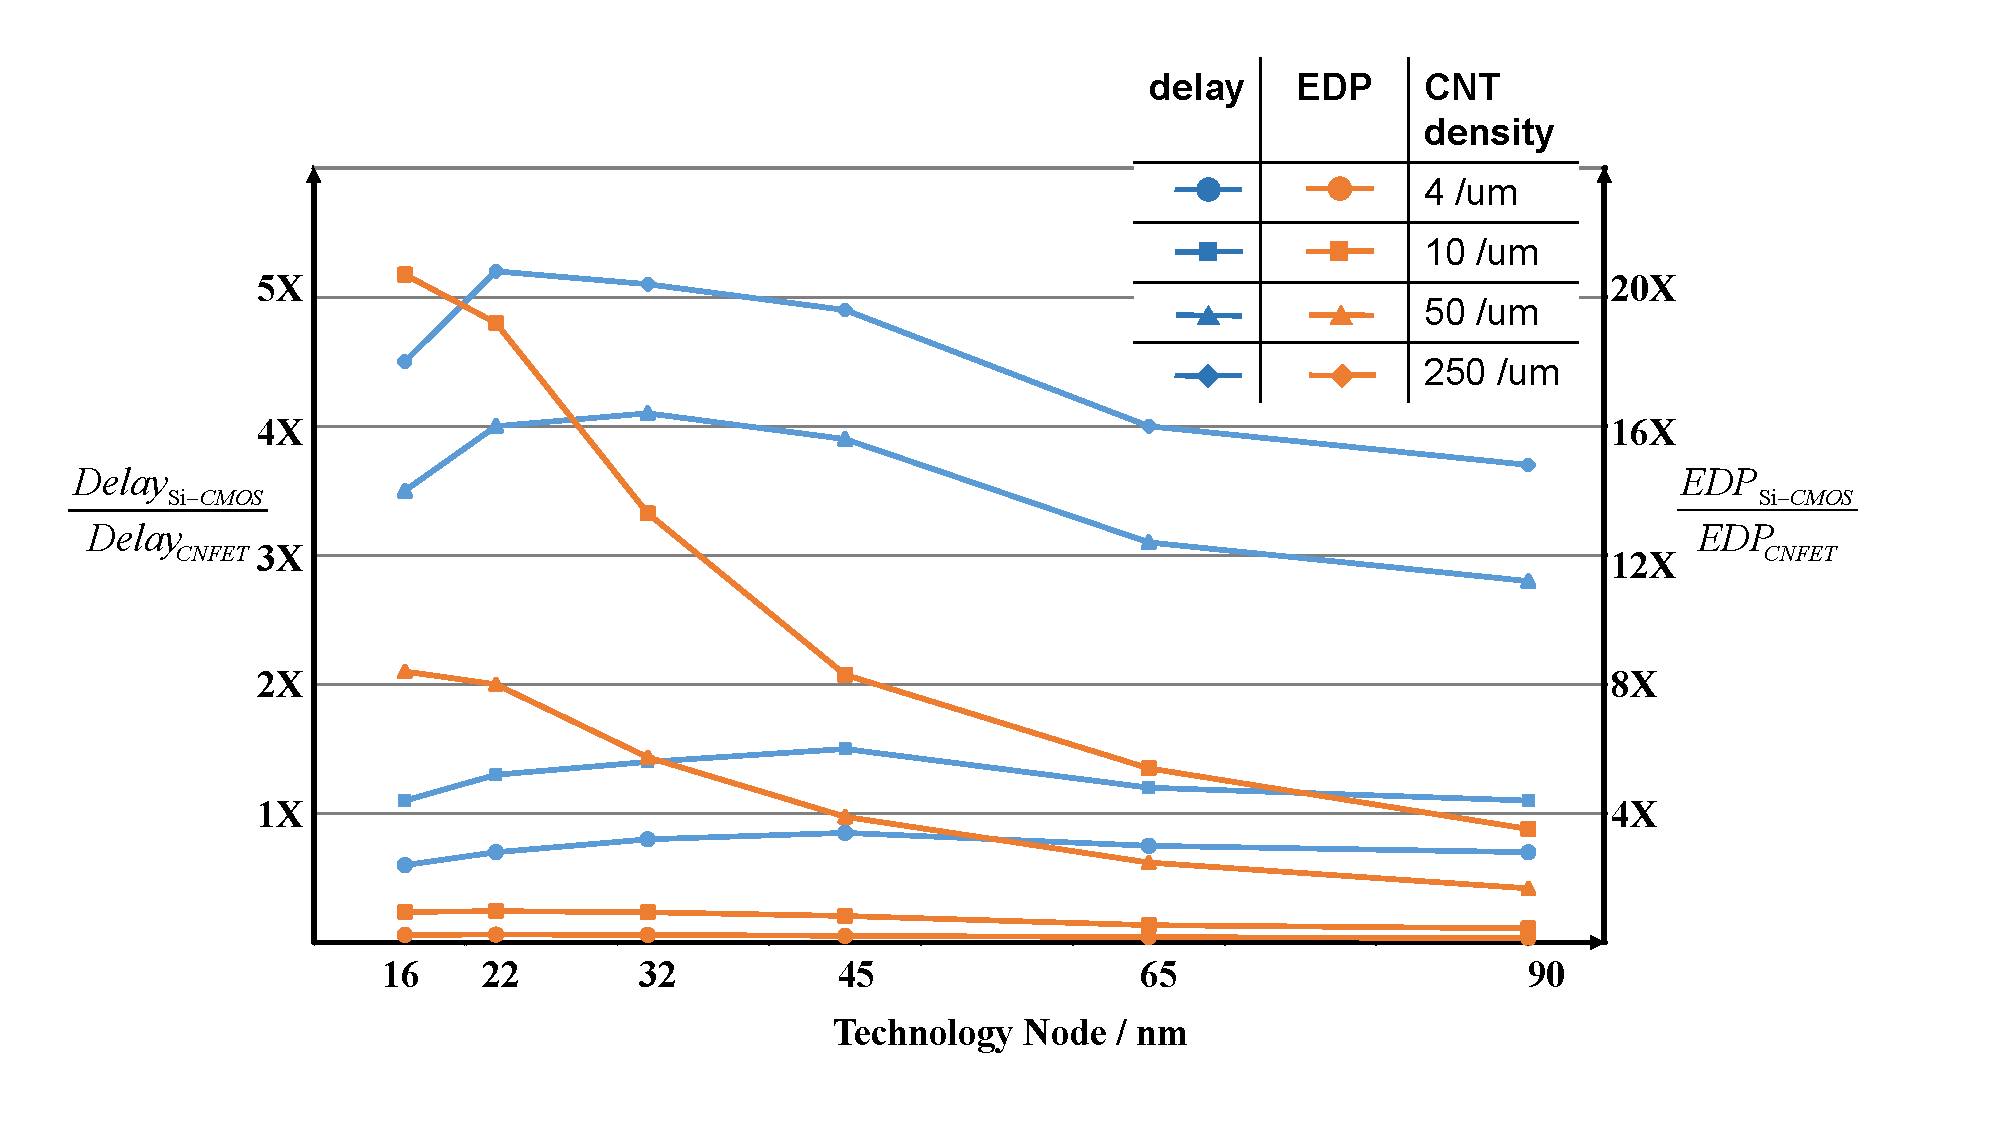
\includegraphics[width=0.95\linewidth]{Density}}
	\center 
        \subfigure[Delay Comparison]{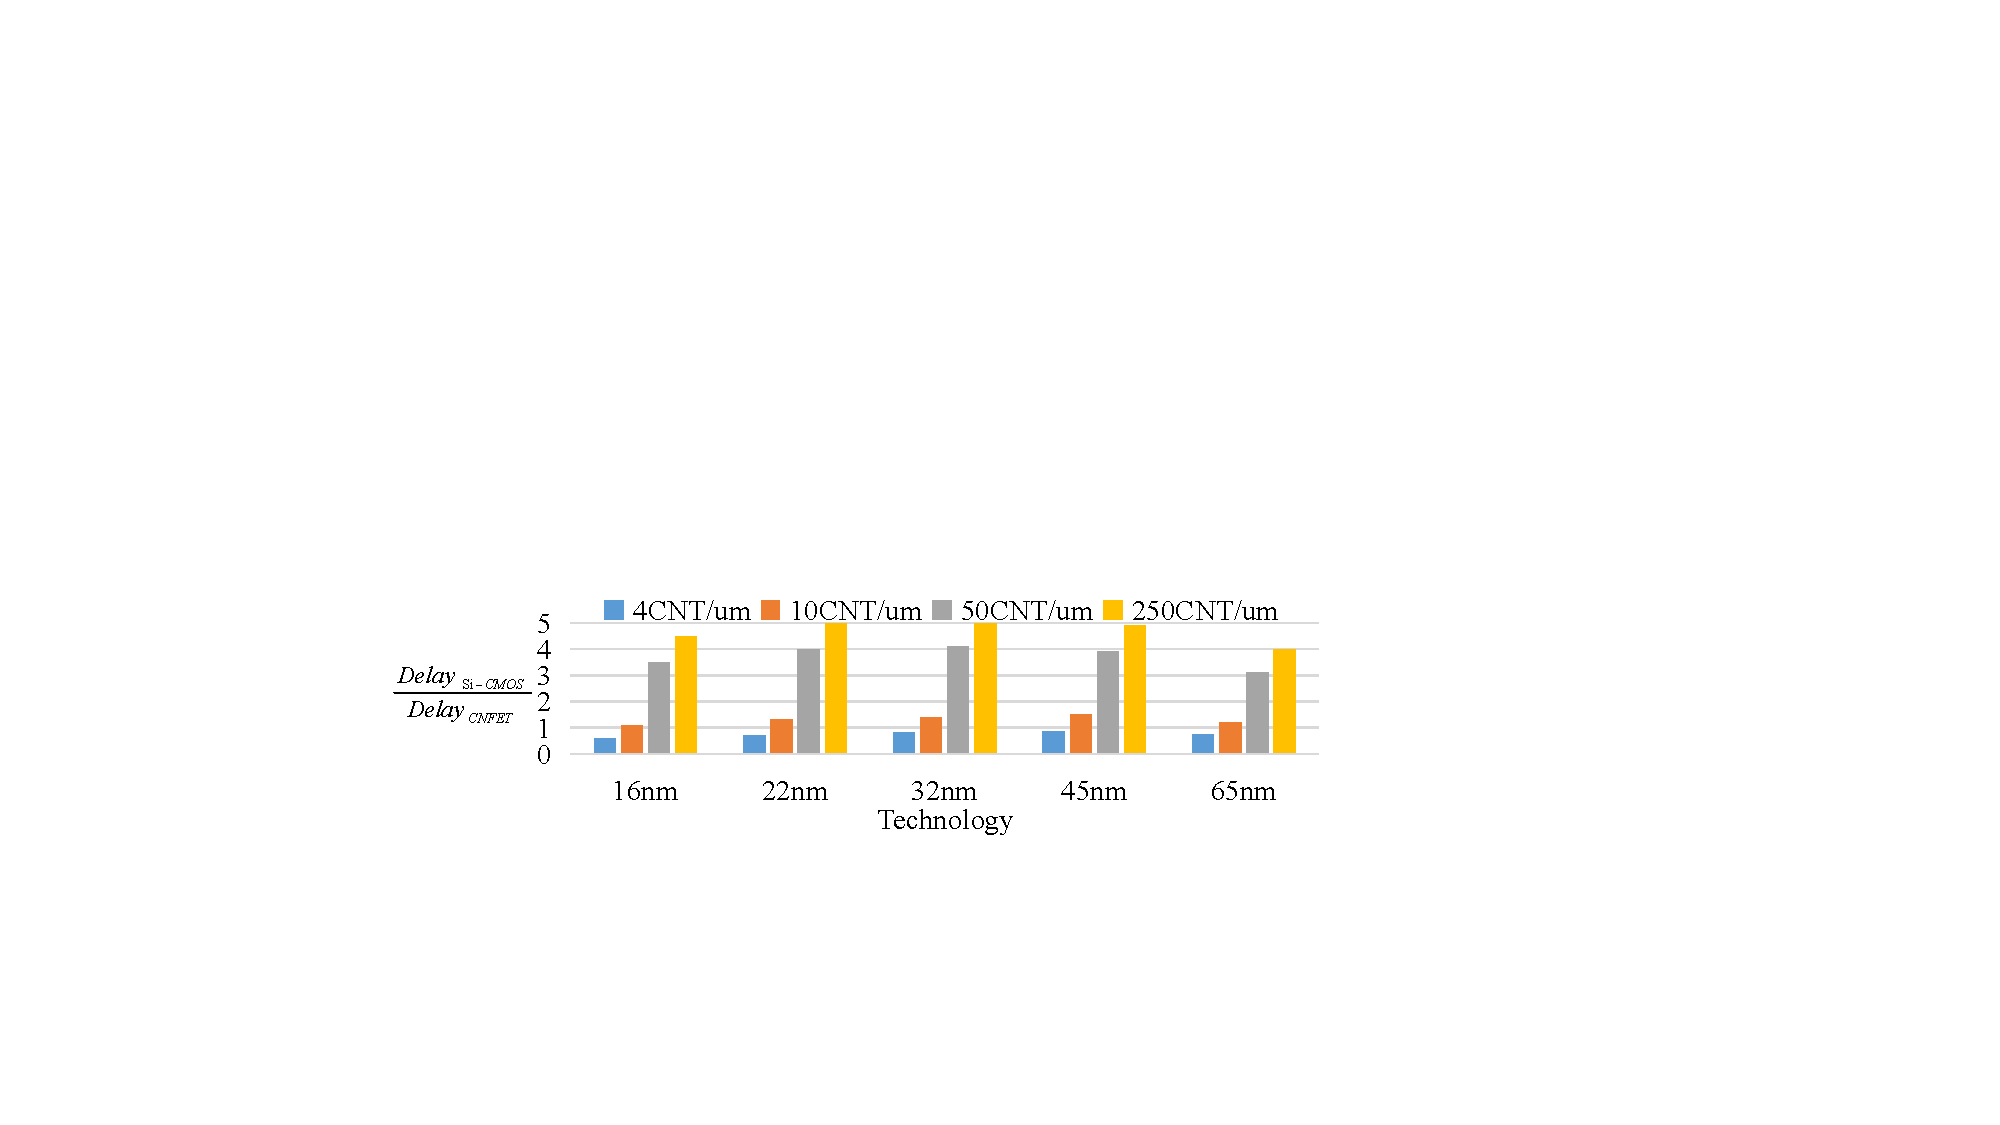
\includegraphics[width=0.85\linewidth]{Delay}}
        \subfigure[Energy Efficiency Comparison]{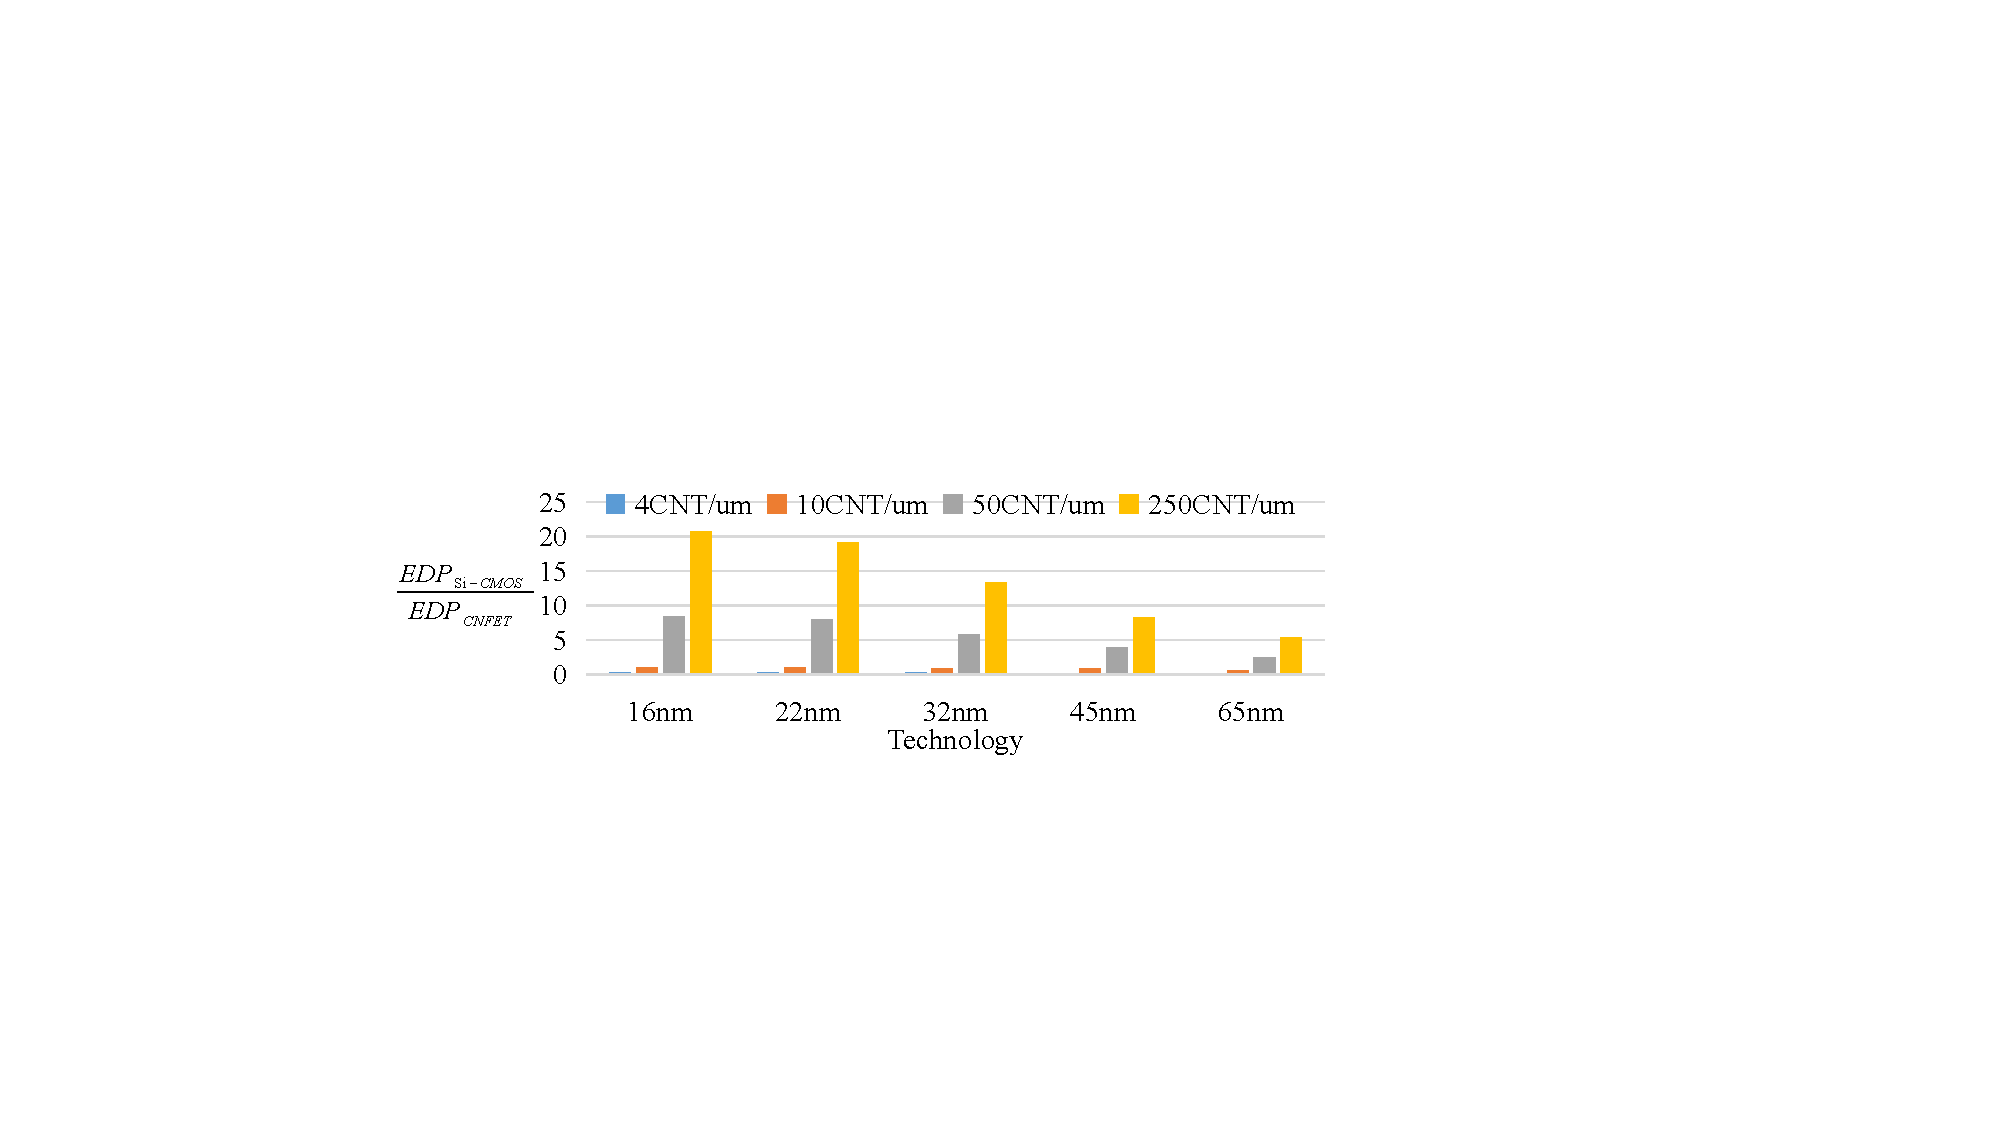
\includegraphics[width=0.85\linewidth]{EDP}}
    \caption{Comparison between CNFET transistors and CMOS transistors under different technologies\cite{patil2008circuit,patil2009digital}}
\label{fig:EDP-advantage}
\vspace{-1em}
\end{figure}


The high operation speed and energy efficiency of CNFET transistors 
make it particularly suitable for power-hungry cache design. 
There are already a large number of SRAM designs using CNFET technology as
proposed in \cite{zhang2012sram, kim2008low, sun2014novel, 
maruthamuthu2013ultra, zhang2011low, sun2017high, sun2018metallic}, which 
can be potentially utilized for cache design. Table \ref{tab:rw-analysis} exhibits 
the detailed operation latency and energy consumption of a typical 
CNFET-based 9-cell SRAM structure \cite{sun2017high,sun2018metallic}. 
The SRAM is a 32$\times$32 bit array fabricated with \SI{16}{nm} technology.
The maximum accessing latency is less than \SI{0.1}{ns} and fulfills the requirements of 
L1 cache in even high-speed processors. Meanwhile, we observe that 
the energy consumption of reading '0' is around 3$\times$ higher 
than that of reading '1'. In contrast, writing '1' consumes almost 10$\times$ 
more energy compared to writing '0'. It indicates that the number of '0' 
and '1' in a data block may lead to distinct SRAM access energy consumption. 

\begin{table}
    \centering
    \label{tab:rw-analysis}
	\caption{Read/Write characteristics of 9T CNFET-based SRAM design\cite{sun2017high}.}
  \label{tab:characteristic-SRAM}
  \begin{tabular}{ccccc}
    \toprule
      Parameters & Read 1 
      & Read 0 
      & Write 1 
      & Write 0 \\
    \midrule
	Delay/ps & 93.65 & 93.65 & 74.36 & 9.12 \\
	Energy/fJ & 1.87 & 4.37 & 2.68  & 0.26 \\
  \bottomrule
\end{tabular}
\vspace{-1em}
\end{table}

With this observation, we may encode a cache line based on the operation type 
and the 0-1 distribution such that the cache operation consumes less energy. 
While the data in a cache line typically changes with time, we develop an adaptive 
encoding module to adapt to the data variation in a cache line. However, changing the 
data encoding and updating the data in a cache line for every single access 
requires non-trivial energy consumption and may also neutralize the benefit of optimized 
data encoding. To that end, we opt to perform the encoding for a window of cache accesses 
instead of a single cache access, which can avoid frequent encoding switch.

The access pattern of a cache line in a window can be either read 
intensive or write intensive. %so the encoding has only two options.
We define the encoding options as encoding directions.
While we cannot block the cache access until the encoding direction is determined, 
we predict the encoding for the next cache access window based on current 
cache data and the latest cache access history. When the predicted encoding direction
differs from the existing encoding direction, the cache line data will be re-encoded 
through inverting such that the 0-1 distribution of the data can be changed to fit 
the cache access preferences. Basically, we inspect the cache line encoding direction 
with the granularity of a window. The encoding may change at runtime when the 
cache access pattern of the window alters. 

We implemented the proposed CNT-Cache with adaptive cache line encoding in 
gem5\cite{binkert2011gem5}. With comprehensive experiments on 
a set of programs from spec2006 and splash2, we demonstrate that CNT-Cache 
takes advantage of the CNFET features and improves the cache energy 
consumption significantly. The contributions are summarized as follows.
\begin{itemize}
    \item With the observation that CNFET-based SRAM have distinct energy
    consumption when accessing '0' and '1', we proposed a novel CNFET-based cache structure 
    which encodes the data at runtime to match the preference of the cache access patterns.
    
    \item We proposed a window-based encoding direction predictor 
    which predicts the encoding direction efficiently based on a window 
    of the latest cache access history. The predictor can be used to guide 
    the cache line encoding at runtime. The predictor and the runtime 
    cache line encoder ensure an energy-efficient CNFET-based cache design.
    
    \item Finally, we implemented the proposed CNT-Cache in gem5 and experimented with both 
    Spec2006 and splash2 benchmarks. The evaluation results show that a D-cache using 
    CNT-Cache structure reduces the energy consumption by 22.2\% on average compared to 
    the baseline cache design.
\end{itemize}

The rest of the paper is organized as follows. In Section \ref{sec:relatedwork},  
we introduce the related work of CNFET-based cache design. 
In Section \ref{sec:warp}, we detail the proposed CNT-cache architecture and the 
optimizations. In Section \ref{sec:result}, we present experiments 
and demonstrate the energy efficiency of CNT-Cache. Finally, we conclude this 
work in Section \ref{sec:conclusion}.

